\documentclass{article}
\usepackage[landscape, margin=0.5cm]{geometry}
\usepackage{multicol}

\usepackage{helvet} % Use Helvetica font (similar to Arial)
\renewcommand{\familydefault}{\sfdefault} % 기본 글꼴을 sans-serif로 설정

\usepackage{amsmath, amsthm}

% Define a new theorem style
\newtheoremstyle{definition}
{1em} % Space above
{0.5em} % Space below
{\normalfont} % Body font
{} % Indent amount
{\bfseries} % Theorem head font
{} % Punctuation after theorem head
{0cm} % Space after theorem head
{\llap{\thmname{#1} \thmnumber{#2}\hskip1em}\thmnote{#3\vspace{0.5em}\newline}}

% Apply the new style to the definition environment
% \theoremstyle{definition}
\theoremstyle{definition}


% Define a custom definition environment
\newtheorem{definition}{Definition}[section]
\newtheorem{theorem}[definition]{Theorem}
\newtheorem{example}[definition]{Example}
\newtheorem{exercise}{Exercise}[section]
\newtheorem*{remark}{Remark}
\newtheorem*{corollary}{Corollary}

% Customize the section style
\usepackage{titlesec}
% \titleformat{\section}[block]
% {\normalfont\large\bfseries}
% {\llap{Section \thesection.0\hskip1em}}{0pt}{}

\renewcommand{\thesubsection}{\arabic{subsection}}
\titleformat{\subsection}[block]
{\normalfont\normalsize\bfseries}
{\llap{Concept \thesubsection\hskip1em}}{0pt}{\large}



% enumerate
\usepackage{enumitem}
% \alph*: 소문자 알파벳 (a, b, c, ...)
% \Alph*: 대문자 알파벳 (A, B, C, ...)
% \roman*: 소문자 로마 숫자 (i, ii, iii, ...)
% \Roman*: 대문자 로마 숫자 (I, II, III, ...)

% math font
\usepackage{amsfonts}


% Redefine the proof environment to match the theorem style
\makeatletter
\renewenvironment{proof}[1][(pf)]{%
    \par
    \pushQED{\qed}%
    \normalfont\topsep3pt\relax
    % \normalfont \topsep6\p@\@plus6\p@\relax
    \trivlist
    \item[\llap{\bfseries#1\hskip0em}]
    \leftskip=2.5em
    \def\forward{\item[\llap{\bfseries($\Rightarrow$)\hskip0em}]}
    \def\backward{\item[\llap{\bfseries($\Leftarrow$)\hskip0em}]}
    \newcommand{\step}[1]{\@ifnextchar\bgroup{\step@binary{##1}}{\step@single{##1}}}
    \newcommand{\step@binary}[2]{\item[\llap{(##1) $\Rightarrow$ (##2)\hskip0em}]}
    \newcommand{\step@single}[1]{\item[\llap{(##1)\hskip0em}]}
}{%
    \popQED\endtrivlist\@endpefalse
}
\makeatother

\usepackage{xcolor} % color
\definecolor{softred}{RGB}{239, 41, 41} % softred


\makeatletter
\newenvironment{hardproof}[1][\textcolor{softred}{(pf)}]{%
    \par
    \pushQED{\qed}%
    \normalfont\topsep3pt\relax
    % \normalfont \topsep6\p@\@plus6\p@\relax
    \trivlist
    \item[\llap{\bfseries#1\hskip0em}]
    \leftskip=2.5em
    \def\forward{\item[\llap{\bfseries($\Rightarrow$)\hskip0em}]}
    \def\backward{\item[\llap{\bfseries($\Leftarrow$)\hskip0em}]}
    \newcommand{\step}[1]{\@ifnextchar\bgroup{\step@binary{##1}}{\step@single{##1}}}
    \newcommand{\step@binary}[2]{\item[\llap{(##1) $\Rightarrow$ (##2)\hskip0em}]}
    \newcommand{\step@single}[1]{\item[\llap{(##1)\hskip0em}]}
}{%
    \popQED\endtrivlist\@endpefalse
}
\makeatother


% hyperlink
\usepackage{hyperref}

\newcommand{\diam}{\text{diam }}


% because
\usepackage{amssymb}


% box
\usepackage[most]{tcolorbox}

\newtcolorbox{notebox}[1][]{
    colback=white!0,
    colframe=black,
    sharp corners,
    boxrule=1pt,
    valign=top,
    left=5pt,
    #1
}

%integral
\usepackage{amsmath}

\def\upint{\mathchoice%
    {\mkern13mu\overline{\vphantom{\intop}\mkern7mu}\mkern-20mu}%
    {\mkern7mu\overline{\vphantom{\intop}\mkern7mu}\mkern-14mu}%
    {\mkern7mu\overline{\vphantom{\intop}\mkern7mu}\mkern-14mu}%
    {\mkern7mu\overline{\vphantom{\intop}\mkern7mu}\mkern-14mu}%
  \int}
\def\lowint{\mkern3mu\underline{\vphantom{\intop}\mkern7mu}\mkern-10mu\int}

%Riemann integral
\usepackage{mathrsfs}

% footnote horizontal
\usepackage[para]{footmisc}

\usepackage[most]{tcolorbox}
\usepackage{xcolor}

\definecolor{mintgreen}{HTML}{E0F8E0}
\definecolor{skyblue}{HTML}{D6EBFF}
\definecolor{peach}{HTML}{FFE5B4}


\newtcolorbox[use counter=definition, number within=section]{mydefinition}[1][]{
  colback=peach,        % 배경색
  colframe=peach,       % 경계선 색상 (배경색과 동일하게 설정하여 경계선을 없앰)
  fonttitle=\bfseries,         % 제목의 글씨체를 볼드체로
  title={\thetcbcounter \, Definition%
         \ifstrempty{#1}{}{:\ #1}}, % 제목 서식 설정, 인수 #1이 비어 있지 않으면 ": #1" 추가
  boxrule=0pt,                 % 경계선 두께 설정 (0pt로 설정하여 경계선 없음)
  sharp corners,               % 모서리를 뾰족하게
  coltitle=black,              % 제목 색상
  colbacktitle=peach,      % 제목 배경색 (본문 배경색과 동일)
  enhanced,                    % 박스의 기타 그래픽적 요소들 향상
  toptitle=5pt,
  left=5pt,
  right=5pt,
  bottom=5pt,
}


\newtcolorbox[use counter=definition, number within=section]{mytheorem}[1][]{
  colback=skyblue,
  colframe=skyblue,
  fonttitle=\bfseries,
  title={\thetcbcounter \, Theorem%
  \ifstrempty{#1}{}{:\ #1}},
  boxrule=0pt,
  sharp corners,
  coltitle=black,
  colbacktitle=skyblue,
  enhanced,                    % 박스의 기타 그래픽적 요소들 향상
  toptitle=5pt,
  left=5pt,
  right=5pt,
  bottom=5pt,
}

\newtcolorbox[use counter=definition, number within=section]{mylemma}[1][]{
    colback=mintgreen,
    colframe=mintgreen,
    fonttitle=\bfseries,
    title={\thetcbcounter \, Lemma%
    \ifstrempty{#1}{}{:\ #1}},
    boxrule=0pt,
    sharp corners,
    coltitle=black,
    colbacktitle=mintgreen,
    enhanced,                    % 박스의 기타 그래픽적 요소들 향상
    toptitle=5pt,
    left=5pt,
    right=5pt,
    bottom=5pt,
}

\newtcolorbox[use counter=definition, number within=section]{myproposition}[1][]{
    colback=mintgreen,
    colframe=mintgreen,
    fonttitle=\bfseries,
    title={\thetcbcounter \, Proposition%
    \ifstrempty{#1}{}{:\ #1}},
    boxrule=0pt,
    sharp corners,
    coltitle=black,
    colbacktitle=mintgreen,
    enhanced,                    % 박스의 기타 그래픽적 요소들 향상
    toptitle=5pt,
    left=5pt,
    right=5pt,
    bottom=5pt,
}

\newtcolorbox[use counter=definition, number within=section]{mycorollary}[1][]{
    colback=mintgreen,
    colframe=mintgreen,
    fonttitle=\bfseries,
    title={\thetcbcounter \, Corollary%
    \ifstrempty{#1}{}{:\ #1}},
    boxrule=0pt,
    sharp corners,
    coltitle=black,
    colbacktitle=mintgreen,
    enhanced,                    % 박스의 기타 그래픽적 요소들 향상
    toptitle=5pt,
    left=5pt,
    right=5pt,
    bottom=5pt,
}

\newtheoremstyle{definition}
{0.5em} % Space above
{0.5em} % Space below
{\normalfont} % Body font
{} % Indent amount
{\bfseries} % Theorem head font
{} % Punctuation after theorem head
{1em} % Space after theorem head
{}

\titleformat{\section}[block]
{\normalfont\large\bfseries}
{Section \thesection. }{0pt}{}

\renewcommand{\thesubsection}{\arabic{subsection}}
\titleformat{\subsection}[block]
{\normalfont\normalsize\bfseries}
{}{0pt}{\large}

\makeatletter
\renewenvironment{proof}[1][\textbf{\proofname)}]{%
    \par
    \pushQED{\qed}%
    \normalfont\topsep3pt\relax
    % \normalfont \topsep6\p@\@plus6\p@\relax
    \trivlist
    \item #1
    \def\forward{\item[\llap{\bfseries($\Rightarrow$)\hskip0em}]}
    \def\backward{\item[\llap{\bfseries($\Leftarrow$)\hskip0em}]}
    \newcommand{\step}[1]{\@ifnextchar\bgroup{\step@binary{##1}}{\step@single{##1}}}
    \newcommand{\step@binary}[2]{\item[\llap{(##1) $\Rightarrow$ (##2)\hskip0em}]}
    \newcommand{\step@single}[1]{\item[\llap{(##1)\hskip0em}]}
}{%
    \popQED\endtrivlist\@endpefalse
}
\makeatother

% img
\usepackage{graphicx}
\usepackage{wrapfig}
\usepackage{capt-of}

\begin{document}
\begin{multicols}{2}
\raggedcolumns

\section{HW 1}
\begin{exercise}
[Section 51 exercise 1]
Show that if $h,h':X\to Y$ are homotopic and $k,k':Y\to Z$ are homotopic, then $k\circ h$ and $k'\circ h'$ are homotopic.
\end{exercise}
\begin{proof}
Let $H:X\times I\to Y, K:Y\times I\to Z$ are homotopies between $h,h'$ and $k,k'$ , respectively. Define $H':X\times I\to Y$ by $H'(x,t) = (H(s,t),t)$. Since both $H$ and $t$ are continuous, $H'$ is continuous. Let $F:X\times I\to Z(=K\circ H')$ be given by $F(x,t) = K(H(s,t),t)$. Then
\begin{enumerate}[label={(\alph*)}]
\item $F$ is composition of continuous functions;
\item $F(x,0) = k(h(x))$;
\item $F(x,1)=k'(h'(x))$
\end{enumerate}
Therefore, $F$ is a homotopy between $k\circ h$ and $k'\circ h'$.
\end{proof}

\begin{exercise}
[Section 51 exercise 3]
A space $X$ is said to be \textbf{\emph{contractible}} if the identity map $i_X:X\to X$ is nulhomotopic.
\begin{enumerate}[label={(\alph*)}]
\item Show that $I$ and $\mathbb{R}$ are contractible.
\item Show that a contractible space is path connected.
\item Show that if $Y$ is contractible, then for any $X$, the set $[X,Y]$ has a single element.
\item Show that if $X$ is contractible and $Y$ is path connected, then $[X,Y]$ has a single element.
\end{enumerate}
\end{exercise}
\begin{proof}
\begin{enumerate}[label={(\alph*)}]
\item Define $F_X:X\times I\to I$ by $F_X(x,t) = xt$. If $X=I$, then $F_I$ is continuous, $F_I(x,0) = 0$ , and $F_I(x,1) = x$, for $x\in I$. If $X=\mathbb{R}$, $F_{\mathbb{R}}$ is continuous, then $F_{\mathbb{R}}(x,0) = 0$, and $F_{\mathbb{R}}(x,1)=x$, for $x\in \mathbb{R}$. Therefore, $F_I$ and $F_{\mathbb{R}}$ are homotopies between $i_I$ and $0$ and between $i_{\mathbb{R}}$ and $0$, respectively.
\item Suppose a space $X$ is contractible space. There is a point $p\in X$ such that a contant map $e_p$ and $i_X$ are homotopic. Let $a,b\in X$ be given. We want to show that there exists a curve $c:I\to X$ between $a$ and $b$.  To do this, let $H:X\times I\to X$ be a homotopy between $e_p$ and $i_X$, where $H(x,0) = i_X(x) = x$, $H(x,1)=p$. We see that
\begin{enumerate}[label={(\alph*)}]
\item $H(a,t)$: a path from $a$ to $p$.
\item $H(b,t)$: a path from $b$ to $p$.
\end{enumerate}
If we define $c = H(a,t)*\overline{H(b,t)}$, then $c$ is a path from $a$ to $b$.
\item Suppose $i_Y\simeq e_p$ for some $p\in Y$. Then $f=i_Y\circ f\simeq e_p\circ f = e_p\circ g\simeq i_Y\circ g=g$.
\item Suppose $i_X\simeq e_p$ for some $p\in X$. Then $f=f\circ i_X\simeq f\circ e_p=e_{f(p)}\simeq e_{g(p)}\simeq g\circ i_X=g$. The homotopy equivalence between $e_{f(p)}$ and $e_{g(p)}$ is derived from the path-connectness of $Y$. Define $F:Y\times I\to Y$ by $F(s,t)=c(t)$ where $c$ denote the curve from $f(p)$ to $g(p)$.
\end{enumerate}
\end{proof}

\begin{exercise}
[Section 52 exercise 4]
Let $A\subset X$; suppose $r:X\to A$ is a continuous map such that $r(a)=a$ for each $a\in A$. (The map $r$ is called a \textbf{\emph{retraction}} of $X$ onto $A$) If $a_0\in A$, show that
$$ r_*:\pi_1(X,a_0)\to \pi_1(A,a_0)$$
is surjective.
\end{exercise}
\begin{proof}
Define $r':A\to X$ by $r'(x) = x$. Consider $r\circ r':A\to A$. We easily see that $r\circ r'$ is well-defined and is a identity map. It implies that $r'$ is a right inverse of $r$, which means $r$ is surjective.
\end{proof}

\begin{exercise}
[Section 52 exercise 7]
Let $G$ be a topological group with operation $\cdot$ and identity element $x_0$. Let $\Omega (G,x_0)$ denote the set of all loops in $G$ based at $x_0$. If $f,g\in \Omega (G,x_0)$, let us define a loop $f\otimes g$ by the rule
$$(f\otimes g)(s)=f(s)\cdot g(s).$$
\begin{enumerate}[label={(\alph*)}]
\item Show that this operation makes the set $\Omega (G,x_0)$ into a group.
\item Show that rhis operation induces a group operation $\otimes$ on $\pi_1 (G,x_0)$.
\item Show that the two group operation $*$ and $\otimes$ on $\pi_1(G,x_0)$ are the same.[Hint: Compute $(f*e_{x_0})\otimes (e_{x_0}*g)$]
\item Show that $\pi_1(G,x_0)$ is abelian.
\end{enumerate}
\end{exercise}
\begin{proof}
\begin{enumerate}[label={(\alph*)}]
\item Let $I(=[0,1])$ be the domain of loops in $\Omega(G,x_0)$. Let $f,g\in \Omega(G,x_0)$. Since, for each $s\in I$, both $f(s)$ and $g(s)$ are in $G$, $(f\otimes g)(s)\in G$. Thus the operation is closed in $\Omega(G,x_0)$. If  $f,g,h\in \Omega(G,x_0)$, then $((f\otimes g)\otimes h)(s) =(f(s)\cdot g(s))\cdot h(s) = f(s)\cdot(g(s)\cdot h(s))=(f\otimes (g\otimes h))(s)$, for all $s\in I$, by the associativity of group operation. Furthermore, $e_{x_0}$ is clearly the identity of $\otimes$. Suppose $f\in \Omega(G,x_0)$. Define $g:G\to G$ by $g(x) = x^{-1}$. By the definition of topological group, $g$ is continuous, so is $g\circ f$. Then, $(g\circ f)\otimes f = f\otimes (g\circ f)=e_{x_0}$, which means that $(g\circ f)$ is the inverse element for $f$ of $\otimes$.
\item Given $[f],[g]\in \pi_1(G,x_0)$, define $[f]\otimes [g]$ by $[f\otimes g]$. We have to check whether the operation is well-defined. Suppose $h,h',k,k'\in \Omega(G,x_0)$, $h\simeq h'$, and $k\simeq k'$. Let $H,K$ be the homotopy between $f,f'$ and between $g,g'$, respectively. Define $HK:I\times I\to G$ by $HK(s,t) = H(s,t)\cdot K(s,t)$. By the definition of topological group, $HK$ is continuous. On top of that, $HK(s,0) = h(s)\cdot k(s)$, $HK(s,1)= h'(s)\cdot k'(s)$. Therefore, it is a homotopy between $h\otimes k$ and $h'\otimes k'$.\\
Suppose $[f],[g],[h]\in \pi_1(G,x_0)$. Then $([f]\otimes [g])\otimes [h]=[f]\otimes ([g]\otimes [h]) = [f\otimes g] \times [h] = [(f\otimes g) \otimes h]=[f\otimes (g\otimes h)]=[f]\otimes [g\otimes h]=[f]\otimes ([g]\otimes [h])$. The identity and inverse are followed by (a).
\item Note that for each $f,g \in \Omega_1(G,x_0)$, $$(f*e_{x_0})\otimes (e_{x_0}*g) = \begin{cases}
f(s)\cdot e_{x_0}(s) & \text{for } 0\leq s\leq \frac{1}{2}\\
e_{x_0}(s)\cdot g(s) & \text{for } \frac{1}{2}\leq s\leq 1
\end{cases}= f*g.$$
Theremore, $[f]\otimes [g] = [f*e_{x_0}]\otimes [e_{x_0}*g]=[f*g]=[f]*[g]$.
\item $[f]*[g]=[f*g]=[f*e_{x_0}]\otimes [e_{x_0}*g]=[e_{x_0}*f]\otimes [g*e_{x_0}]=[g*f]=[g]*[f]$, for each $[f],[g]\in \pi_1(G,x_0)$.
\end{enumerate}
\end{proof}

\begin{exercise}
[Section 53 exercise 3]
Let $p:E\to B$ be a covering map; let $B$ be connected. Show that if $p^{-1}(b_0)$ has $k$ elements for some $b_0\in B$, then $p^{-1}(b)$ has $k$ elements for every $b\in B$. In such a case, $E$ is called a \textbf{\emph{k-fold covering}} of $B$. 
\end{exercise}
\begin{proof}
Let $B_0:=\{b\in B\mid |p^{-1}(b)|=k\}$. $B_1:=\{b\in B\mid |p^{-1}(b)\neq b\}$. By hypothesis, $|B_0|\neq 0$. Suppose, for contradiction, $|B_1| \neq 0$. Since $p$ is a covering map, for each element of $B_0$, there exists a open subset $U_\alpha$ of $B$ evenly covered by $p$. Likewise, for $b\in B_1$, there exists $V_\beta\subset B$ evenly covered by $p$, for some integer $n\neq k$. Let $U= \bigcup \{U_\alpha\}$, $V=\bigcup\{V_\beta\}$. Then
\begin{enumerate}[label={(\alph*)}]
\item Since $U$, $V$ are union of open sets, they are open.
\item Clearly $(U\cap B)\cup (V\cap B)=B$.
\item $U\cap V=\varnothing$. Suppose $x\in U\cap V$, then $|p^{-1}(x)| = k = n$, leading to a contradiction.
\end{enumerate}
That is, $U$, $V$ seperate $B$, leading a contradiction. Thus, $B_1$ is an empty set.
\end{proof}

\begin{exercise}
[Section 53 exercise 6]
Let $p:E\to B$ be a covering map.
\begin{enumerate}[label={(\alph*)}]
\item If $B$ is Hausdorff, regular, completely regular, or locally compact Hausdorff, then so is $E$. [Hint: If $\{V_\alpha\}$ is a partition of $p^{-1}(U)$ into slices, and $C$ is a closed set of $B$ such that $C\subset U$, then $p^{-1}(C)\cap V_\alpha$ is a closed set of $E$.]
\item If $B$ is compact and $p^{-1}(b)$ is finite for each $b\in B$, then $E$ is compact.
\end{enumerate}
\end{exercise}
\begin{proof}
(b) Let an open cover $\{U_\alpha\}$ of $E$ be given. For every $b\in B$, there exists $V_b$ evenly covered by $p$. Each $V_b$ has the covering space of finite disjoint open set $W_{b_\beta}$. Consider the intersection of each $U_\alpha$ and $W_{b_\beta}$. Since $p$ is surjective and the set $\{V_b\}$ is an open cover of $B$, the union of every $U_\alpha \cap W_{b_\beta}$ contains $E$. It implies that the union of every $p(U_\alpha \cap W_{b_\beta})$ contains $B$. Therefore, there is a finite subcover $\{p(U_{\alpha_n}\cap W_{b_{\beta_m}})\}$ containing $B$. The preimage of each $p(U_{\alpha_n}\cap W_{b_{\beta_m}})$ is a finite-fold covering of $p(U_{\alpha_n}\cap W_{b_{\beta_m}})$, thus the number of every disjoint open set of preimage of $p(U_{\alpha_n}\cap W_{b_{\beta_n}})$ is also finite, and union of them contains $E$. Since $(U_{\alpha_n}\cap W_{b_{\beta_m}}) \subset U_{\alpha_n}$, $E$ is contains in the union of $\{U_{\alpha_n}\}$. It is a finite subcover of $E$. 
\end{proof}

\columnbreak

\begin{exercise}
[Section 54 exercise 5]
Consider the covering map $p\times p:\mathbb{R}\times \mathbb{R}\to S^1\times S^1$ of Example 4 of setction 53. Consider the path $f(t)=(\cos 2\pi t, sin 2\pi t)\times (\cos 4\pi t,\sin 4\pi t)$ in $S^1\times S^1$. Sketch what $f$ looks like when $S^1\times S^1$ is identified with the doughnut surface $D$. Find a lifting $\overline{f}$ of $f$ to $\mathbb{R}\times \mathbb{R}$, and sketch it.
\end{exercise}
\begin{proof}
Define $\tilde{f}:I\to \mathbb{R}\times \mathbb{R}$ by
$$\tilde{f}(s) = (s,2s).$$
Then $p\circ \tilde{f}=f$. To visualize this, let $g:S^1\times S^1\to \mathbb{R}^3$ given by 
$$g((x_1,y_1)\times (x_2,y_2))=((1+\frac{1}{3}x_1)x_2, (1+\frac{1}{3}x_1)y_2, \frac{1}{3}y_1).$$
Then 
\begin{align*}
    (g\circ p)(u,v) &= g((\cos 2\pi u,\sin 2\pi u)\times (\cos 2\pi v,\sin 2\pi v))\\
        &= ((1+\frac{1}{3}\cos 2\pi u)\cos 2\pi v, (1+\frac{1}{3}\cos 2\pi u)\sin 2\pi v, \frac{1}{3}\sin 2\pi u)
\end{align*}
and
\begin{align}
    (g\circ f)(s) &= g((\cos 2\pi s,\sin 2\pi s)\times (\cos 4\pi s,\sin 4\pi s)) \\
        &= ((1+\frac{1}{3}\cos 2\pi s)\cos 4\pi s, (1+\frac{1}{3}\cos 2\pi s)\sin 4\pi s, \sin 2\pi s)
\end{align}
If we render this using a graphics tool, the result looks like the following image.
\end{proof}
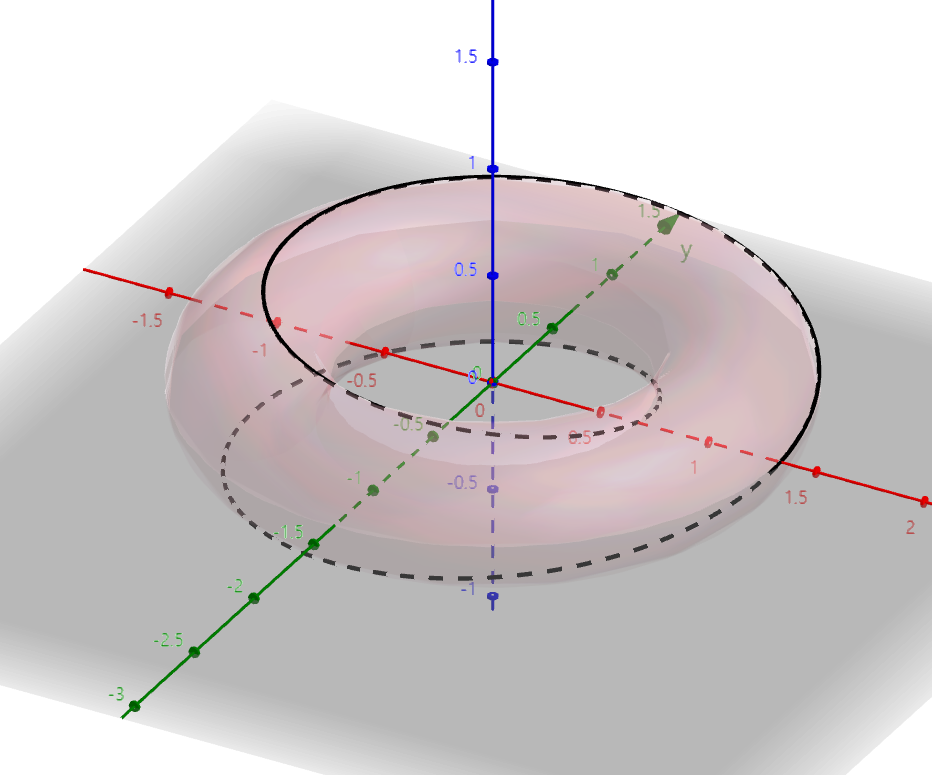
\includegraphics[width=0.9\linewidth]{torus.png}
\captionof{figure}{The path $f$ on the torus $p$}

\begin{exercise}
[Section 54 exersice 6]
Consider the maps $g,h:S^1\to S^1$ given $g(z)=z^n$ and $h(z)=1/z^n$. (Here we represent $S^1$ as the set of complex numbers $z$ of absolute value 1.) Compute the induced homomorphism $g_*$,$h_*$ of the infinite cyclic group $\pi_1(S^1,b_0)$ into itself. [Hint: Recall the equation $(\cos \theta + i\sin \theta)^n = \cos n\theta + \sin n\theta$.]
\end{exercise}
\begin{proof}
Since $S^1$ is path-connected, $\pi_1(S^1,b_0)\cong \pi_1(S^1,(1,0))$. We may assume $b_0=(1,0)$. Let $f:I\to S^1$ given by $f(t)=(\cos 2\pi t, \sin 2\pi t) = e^{2\pi it}$. Then $f(0) = f(1) = (1,0)$, and the equivalence class $[f]\in \pi_1(S^1,(1,0))\cong \mathbb{Z}$ corresponds to $1\in \mathbb{Z}$, so it is a gererater of $\pi_1(S^1,(1,0))$. Define a isomorphism $\phi:\pi_1(S^1,(1,0))\to \mathbb{Z}$ by $\phi([e^{2\pi nt}])=n$. Then $(\phi \circ g_*)([f]) = \phi([g\circ f])=\phi([e^{2\pi nt}])=n$. Since $[f]$ is a generator of $\pi_1(S^1,(1,0))$, $n$ is a generator of $(\phi \circ g_*)(\pi_1(S^1,(1,0)))$, $n \mathbb{Z}$. Consequently, $g_*(\pi_1(S^1,(1,0)))\cong (\phi \circ g_*)(\pi_1(S^1,(1,0))) = n \mathbb{Z}$. Similarly, $h_*(\pi_1(S^1,(1,0))) \cong (\phi \circ h_*)(\pi_1(S^1,(1,0))) = -n \mathbb{Z}$.
\end{proof}

\clearpage

\section{HW2}
$\varnothing$


\end{multicols}
\end{document}
